\section{The temperature monitoring system of ProtoDUNE-SP}
\label{sec:protoDUNE}

\noindent ProtoDUNE-SP~\cite{pdsp_tdr} was the single-phase (SP) demonstrator of DUNE far detector second module \cite{dune_tdr4}, currently known as Horizontal Drift (HD) module. %It was built at the CERN Neutrino Platform and, with a total LAr mass of 0.77 kt, it represents the largest monolithic LArTPC detector built to date. 
The elements constituting the TPC, its associated readout electronics and the photon detection system, were housed in a 8x8x8 m$^3$ cryostat that contained the LAr target material. The cryostat, a free-standing steel-framed vessel with an insulated double membrane, is based on the technology used for liquefied natural gas storage and transport. A cryogenic system maintains the LAr at a stable temperature of about 87 K, and ensures the required purity level by means of a closed-loop process that recovers the evaporated argon, recondenses it, filters it, and returns it to the cryostat, keeping the LAr level at about 7.3 m from the bottom membrane. ProtoDUNE-SP was exposed to a charged particle test-beam from October to November 2018, and later recorded cosmic rays until January 2020 \cite{pdsp_1,pdsp_2}. It was finally emptied and decommissioned in Summer 2020.

In order to understand the LAr behaviour inside the cryostat and validate the CFD simulations, 92 high-precision temperature sensors were installed inside ProtoDUNE-SP, near the active volume. These sensors were distributed in two vertical arrays, or Temperature Gradient Monitors (TGM), and two horizontal grids below and above the TPC, respectively. Three elements were common to all systems: sensors, cables and readout electronics. RTD technology \cite{minco} was chosen for this application. It consists of a metallic element whose resistance changes with temperature. This resistance is measured by feeding the RTD with a known current and measuring the resulting voltage. Based on previous experience from other prototypes \cite{35t_1}, Lake Shore PT102 platinum sensors \cite{pt102} with 100 ohms resistance at room temperature were chosen. Sensors were mounted on a 52x14 mm$^2$ PCB with an IDC-4 connector, such that they could be plugged-in at any time. Several versions of the PCB have been explored, finally converging to the one shown in Fig.~\ref{fig:sensor}, which minimizes the contact of the sensor with the PCB while keeping the sensor protected. 

\begin{figure}[htbp]
\begin{center}
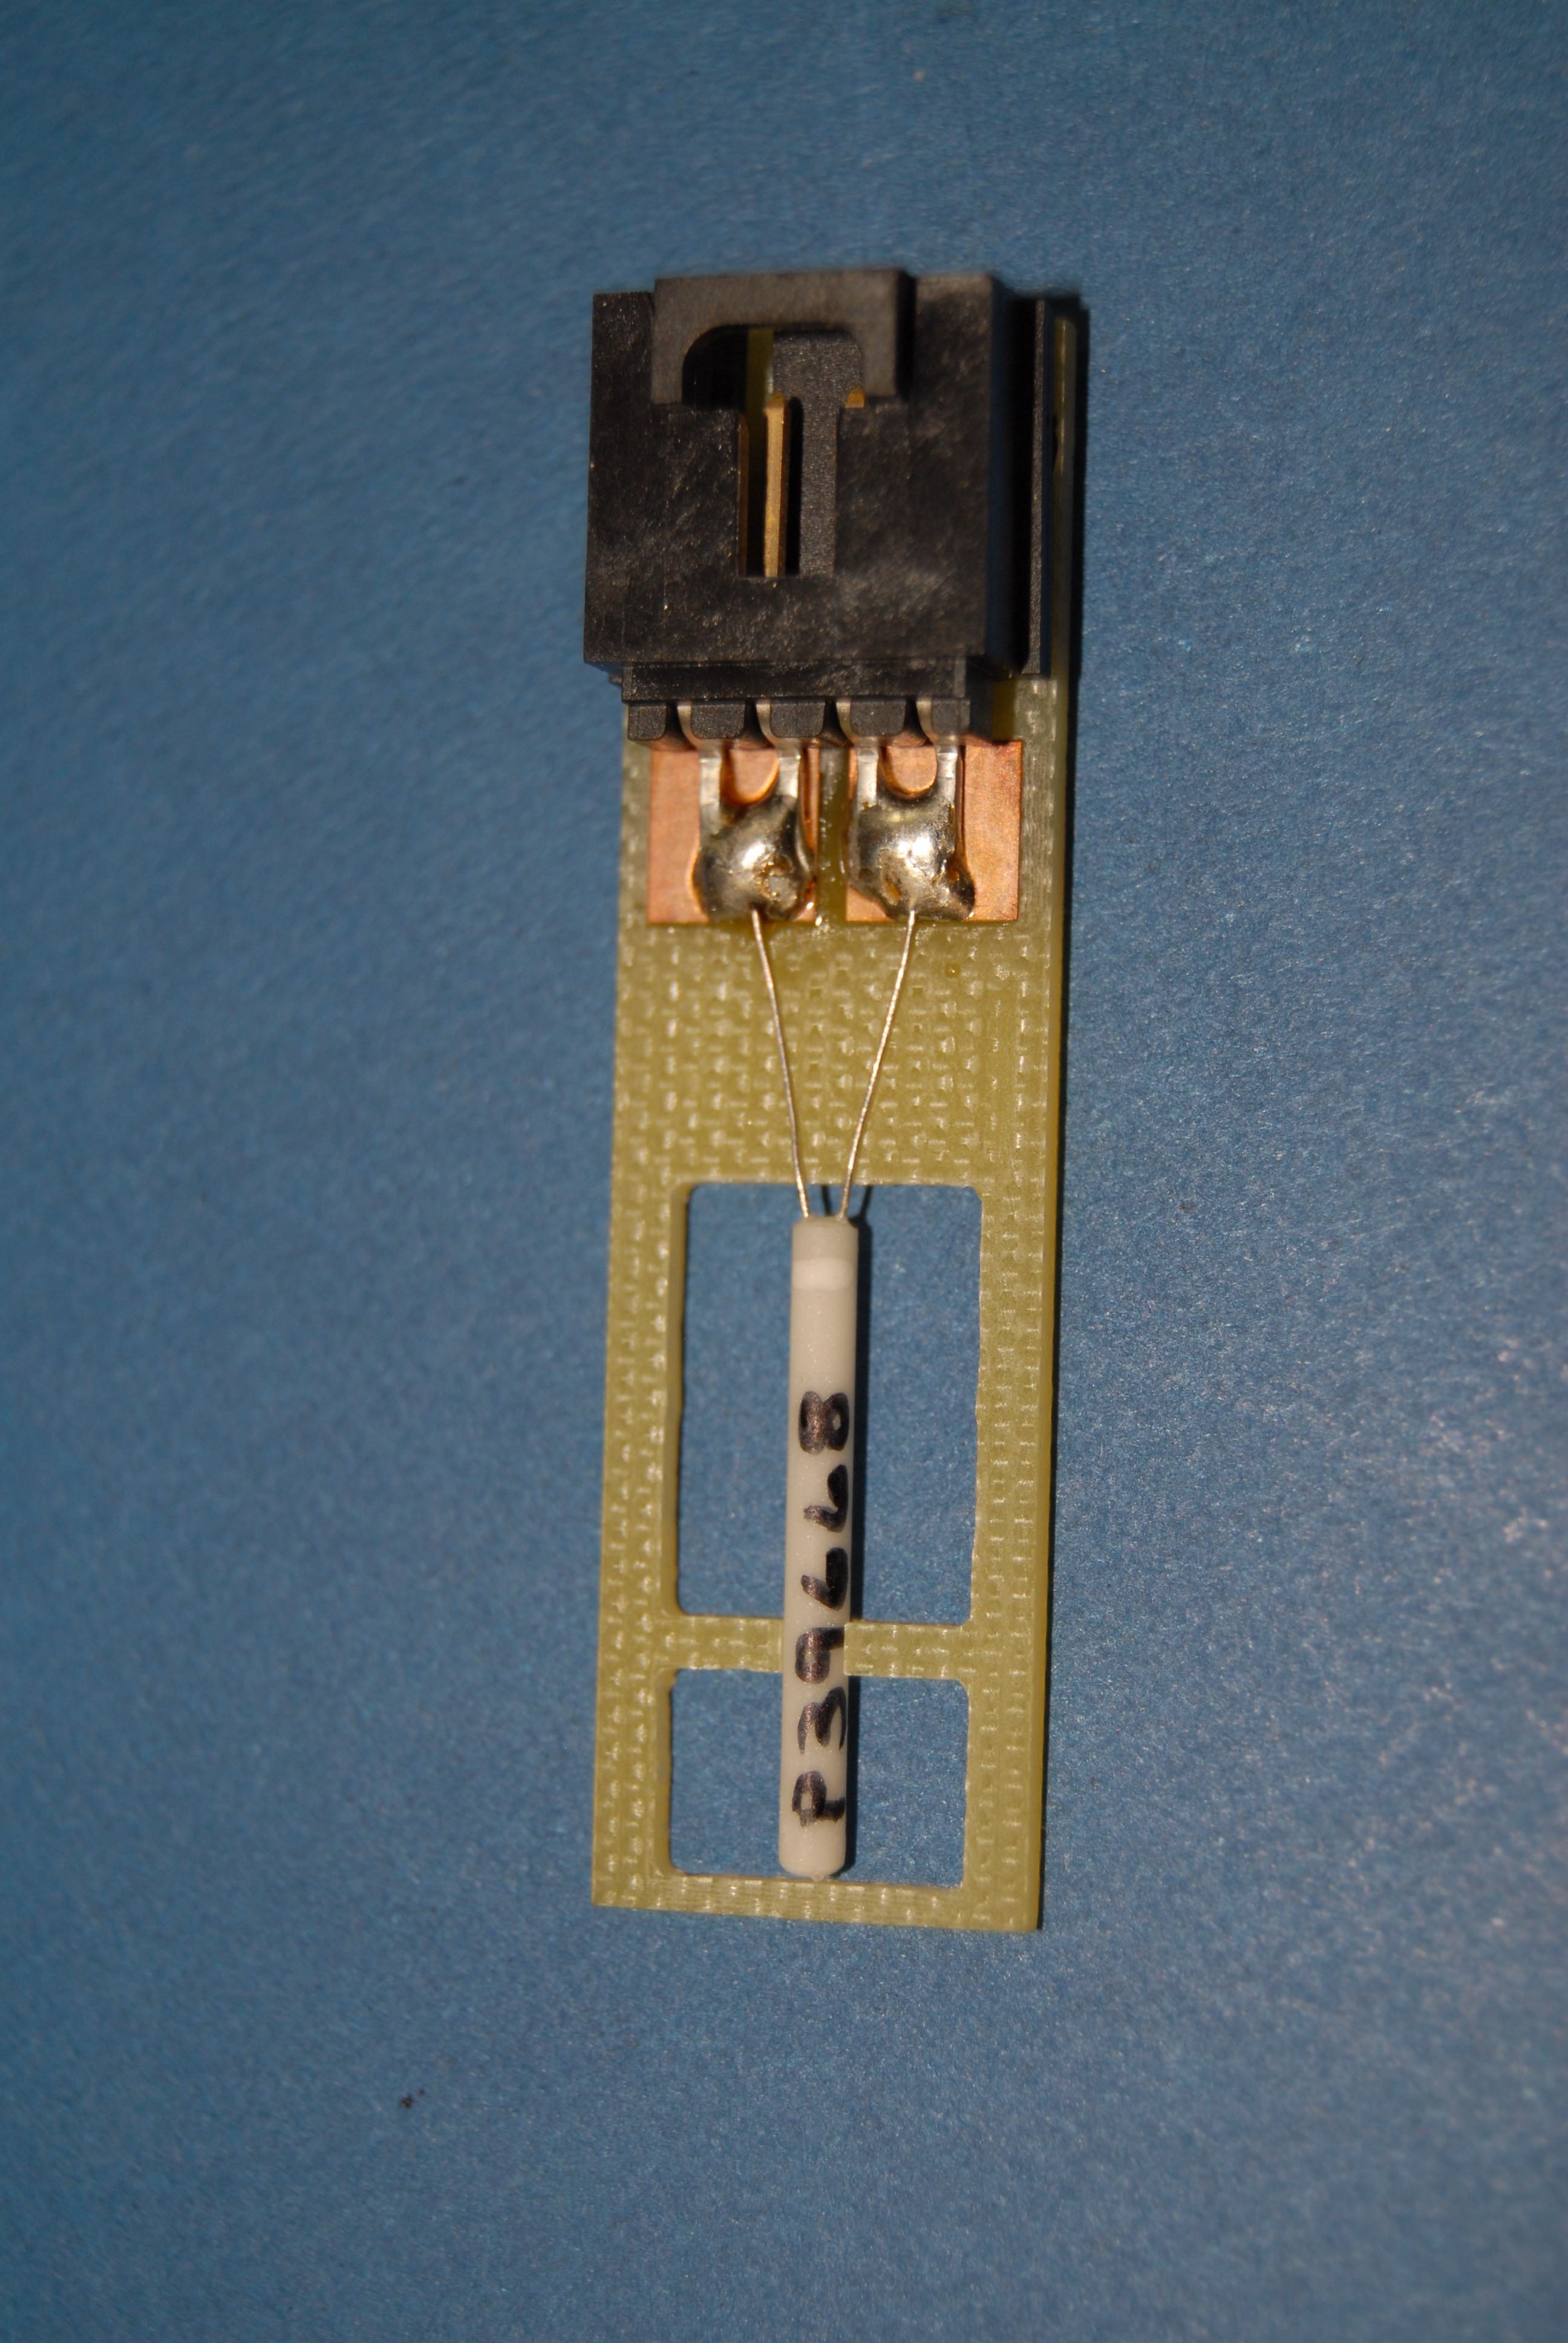
\includegraphics[width=0.6\textwidth, angle=-90]{images/figure_1.jpg}%
\caption{PCB support with temperature sensor and IDC-4 connector. The transition from two wires at the sensor to 4 wires at the readout is clearly seen. The sensor has a length of 2 cm.
\label{fig:sensor}}
\end{center}
\end{figure}

A careful choice of the readout cable and the proper connections are essential to obtain the required temperature precision. See for example \cite{minco} for a detailed description. A custom cable made by Axon \cite{axon} was used. It consists of four American Wire Gauge (AWG) 28 teflon-jacketed copper wires, forming two twisted pairs, with a metallic external shield and an outer teflon jacket. The outer diameter of the cable is 3.7 mm. Teflon was chosen for its good thermal properties and low out-gassing. The metallic external shield (connected to the readout in one end and left floating at the sensor's end) and the twisted pairs are crucial to reduce the effect of external electromagnetic noise pickup. When RTDs are far from the voltmeter, the resistance of cables and connectors are added to the one of the sensor, biasing the temperature measurement. This bias can be subtracted to some level, but cannot be fully controlled since the resistance of those elements also depends on temperature. To minimise the impact of this effect a four wire readout is introduced \cite{minco}, such that the voltage is measured in the vicinity of the RTD.  

The last common element is the readout system, consisting of a very precise 1 mA current source to excite the sensors and a 24 bits ADC to measure the voltage. The readout system will be described in detail in section \ref{sec:readout}. 

As previously mentioned, ProtoDUNE-SP CFD simulations predict vertical temperature gradients as low as 15 mK \cite{pdsp_tdr}. A relative precision better than 5 mK was required to validate and tune those simulations with sufficient confidence. Three main ingredients are necessary to obtain such a precision: i) high quality and stable temperature probes, ii) a very precise readout system, and iii) a proper calibration, both for the readout and the sensors. As mentioned above, two TGMs were deployed in ProtoDUNE-SP: one could be moved vertically and hence calibrated \textit{in situ}, while the other one ---static--- fully relied on a prior calibration in the laboratory. In this article, the calibration of the static TGM \cite{tfm} sensors is be described in detail. This device consists of a vertical array of 48 sensors, installed 20 cm away from the lateral field cage. 

The calibration was performed once in spring 2018  (a few months before the operation of ProtoDUNE-SP), and several times after ProtoDUNE-SP decommissioning. In this article the calibration setup, procedure and results will be described in detail. Comparison between the different calibration campaigns will be addressed, revealing important information about systematic uncertainties and RTD ageing.